% this file is called up by thesis.tex
% content in this file will be fed into the main document

%: ----------------------- name of chapter  -------------------------
\chapter{Experimental Environment and Experiments} % top level followed by section, subsection


%: ----------------------- paths to graphics ------------------------

% change according to folder and file names
\ifpdf
    \graphicspath{{X/figures/PNG/}{X/figures/PDF/}{X/figures/}}
\else
    \graphicspath{{X/figures/EPS/}{X/figures/}}
\fi

%: ----------------------- contents from here ------------------------


This chapter introduces the experimental environment and how the environment was designed and developed to receive results, which do not include overhead from the Operating System and support time measurements with nano-second accuracy. The chapter also describes the experiments that are used in the practical part of this project. The experiments were developed because described in section \ref{sec:benchmarks} benchmarking tools cannot provide precise and trustworthy information to parametrise the model. Both this chapter and chapter \ref{chapterCondExp} contain a great number of details; it should allow a reader to replicate the study, if required.

Figure \ref{exp_env_exp} outlines the structure of the proposed solution. This part of the document starts from describing the file structure, which lies in the base of all elements of the solution. The experimental environment is used to set-up the laboratory setting that is capable of monitoring unwanted events imposed by the OS and provide accurate time measurements with nano-second level of accuracy. A number of cycle- and application-level experiments are executed from the experimental environment. Gathered from running experiments data is recorded into CSV files / outputted on the screen by the experimental environment.

\begin{figure}[ht!]
\centering
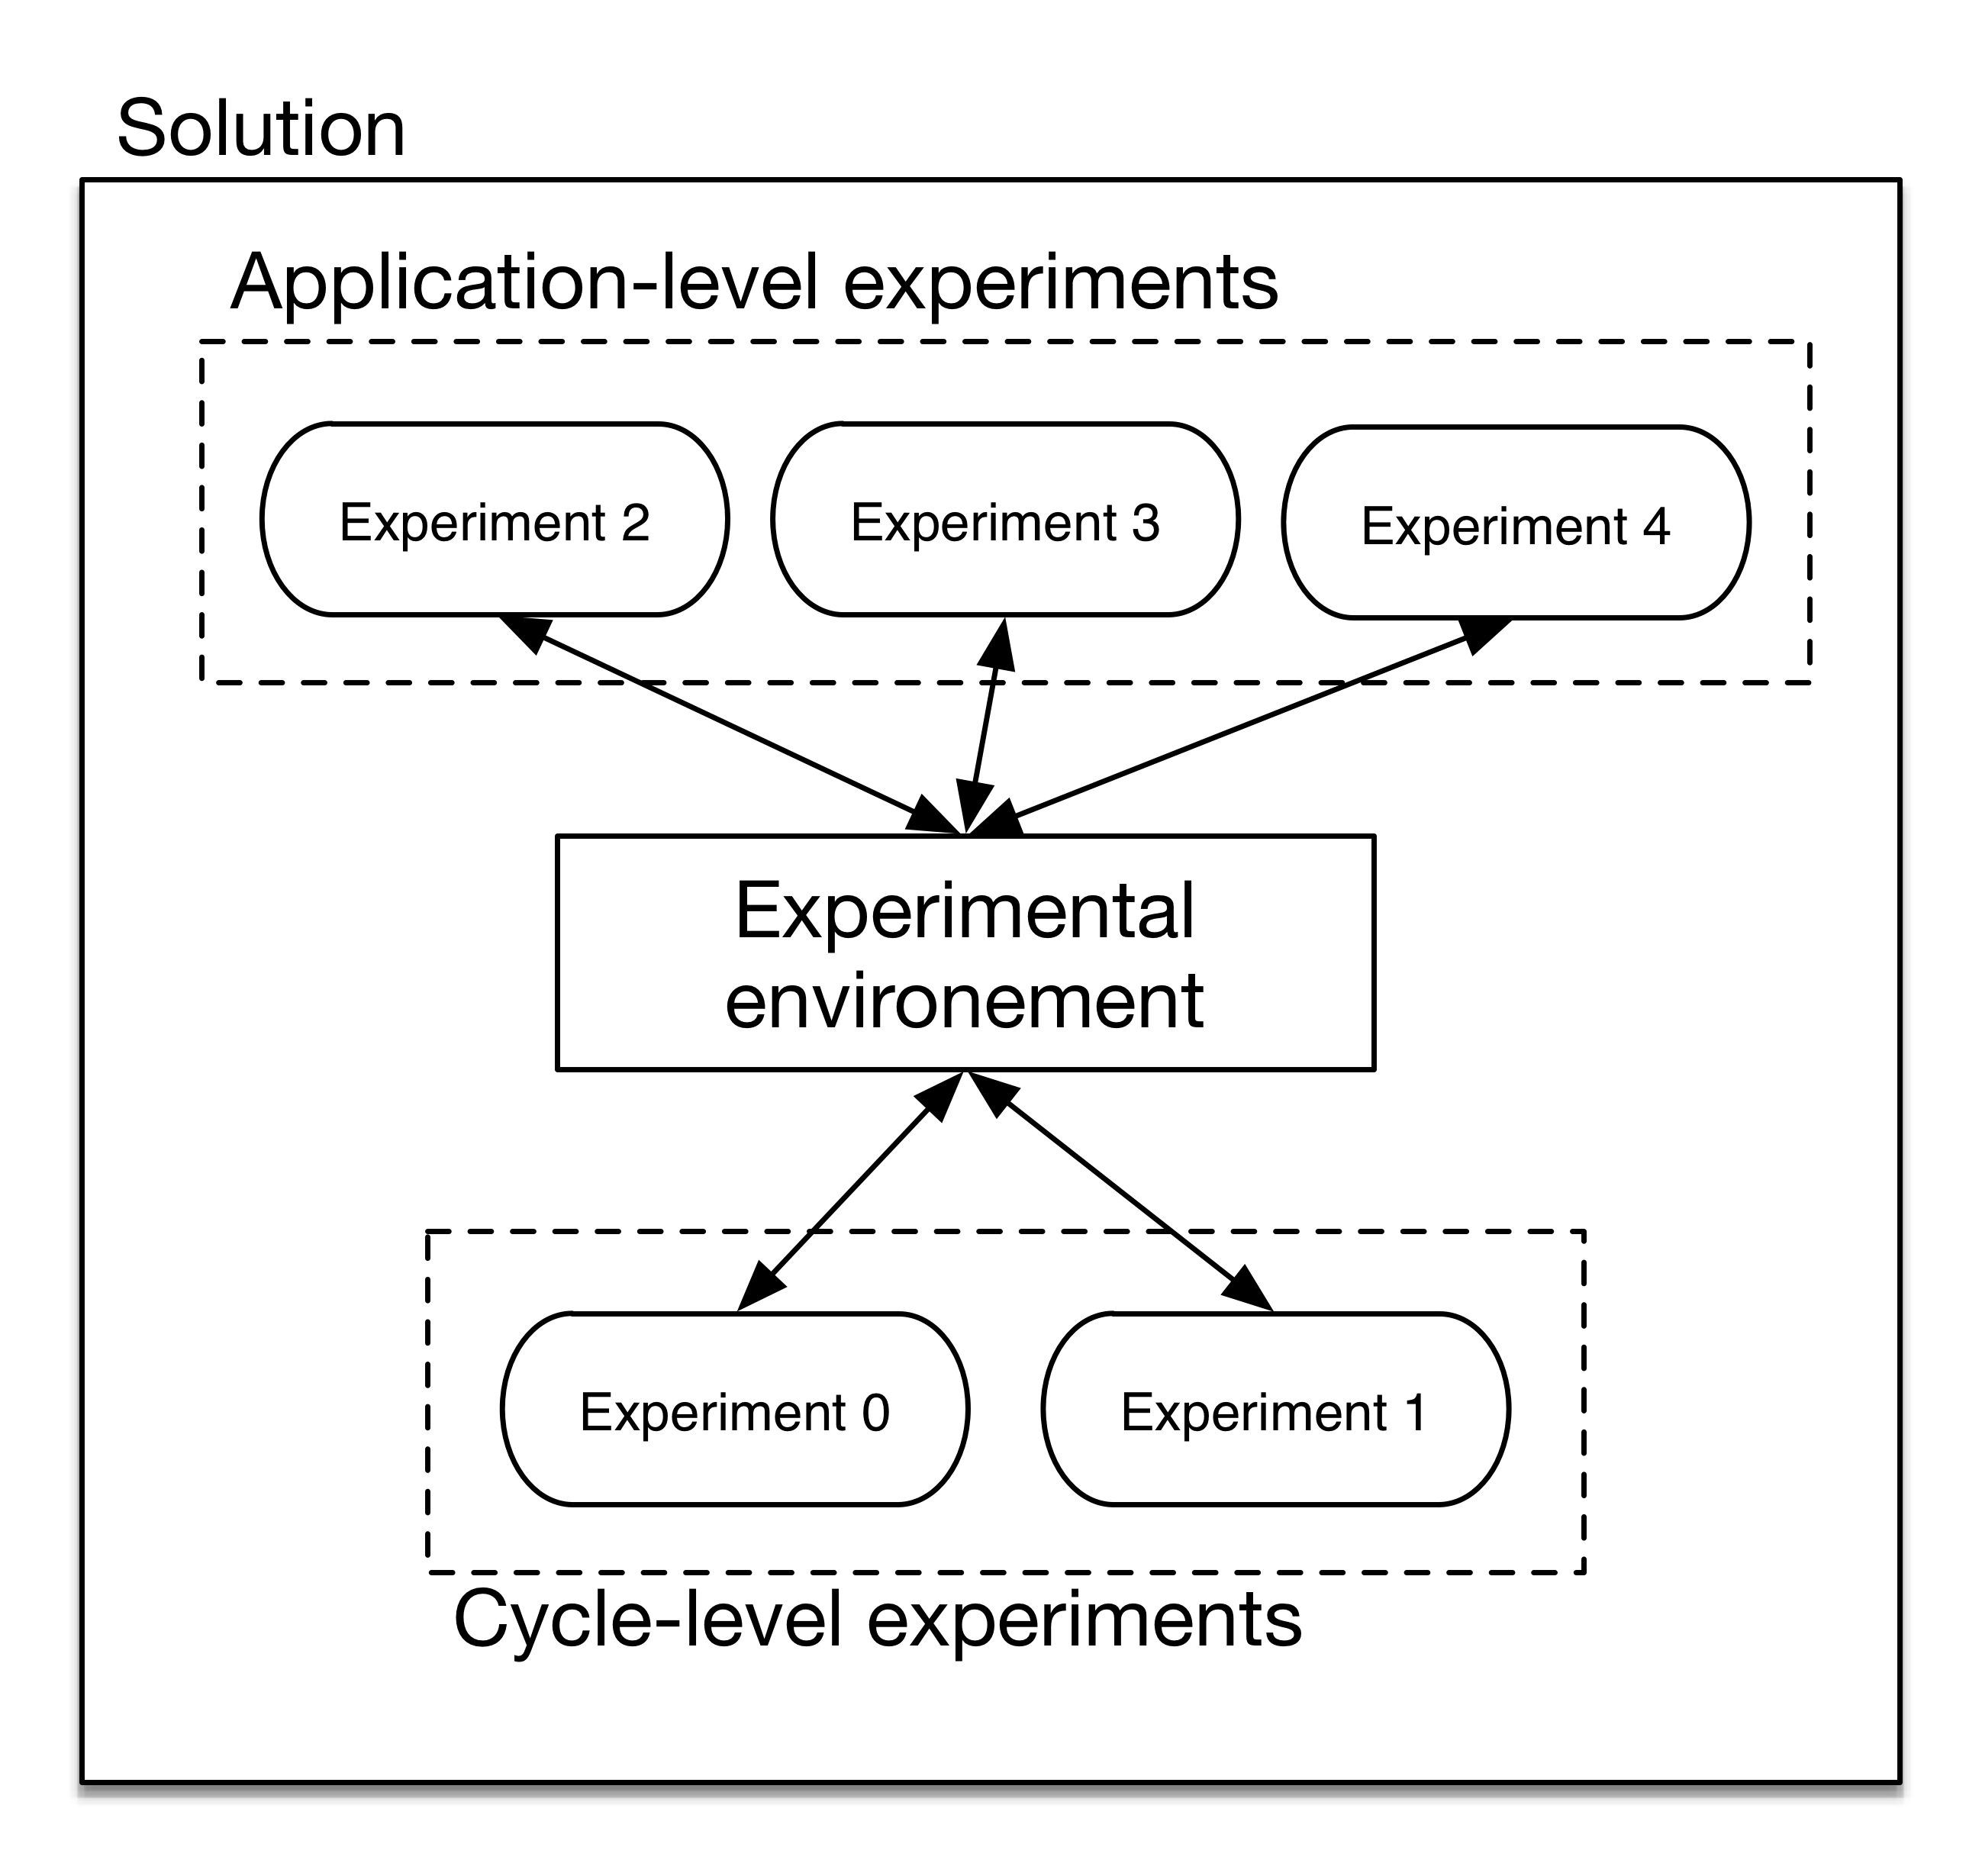
\includegraphics[width=90mm]{4/exp_env_exp.png}
\caption{Overview of the solution}
\label{exp_env_exp}
\end{figure}

Refer to the flowchart \ref{flowExperiment}, it outlines the actions that take place when experiments are run. The sections of this chapter give a detailed description of all processes that are present on the figure.

\begin{figure}[ht!]
\centering
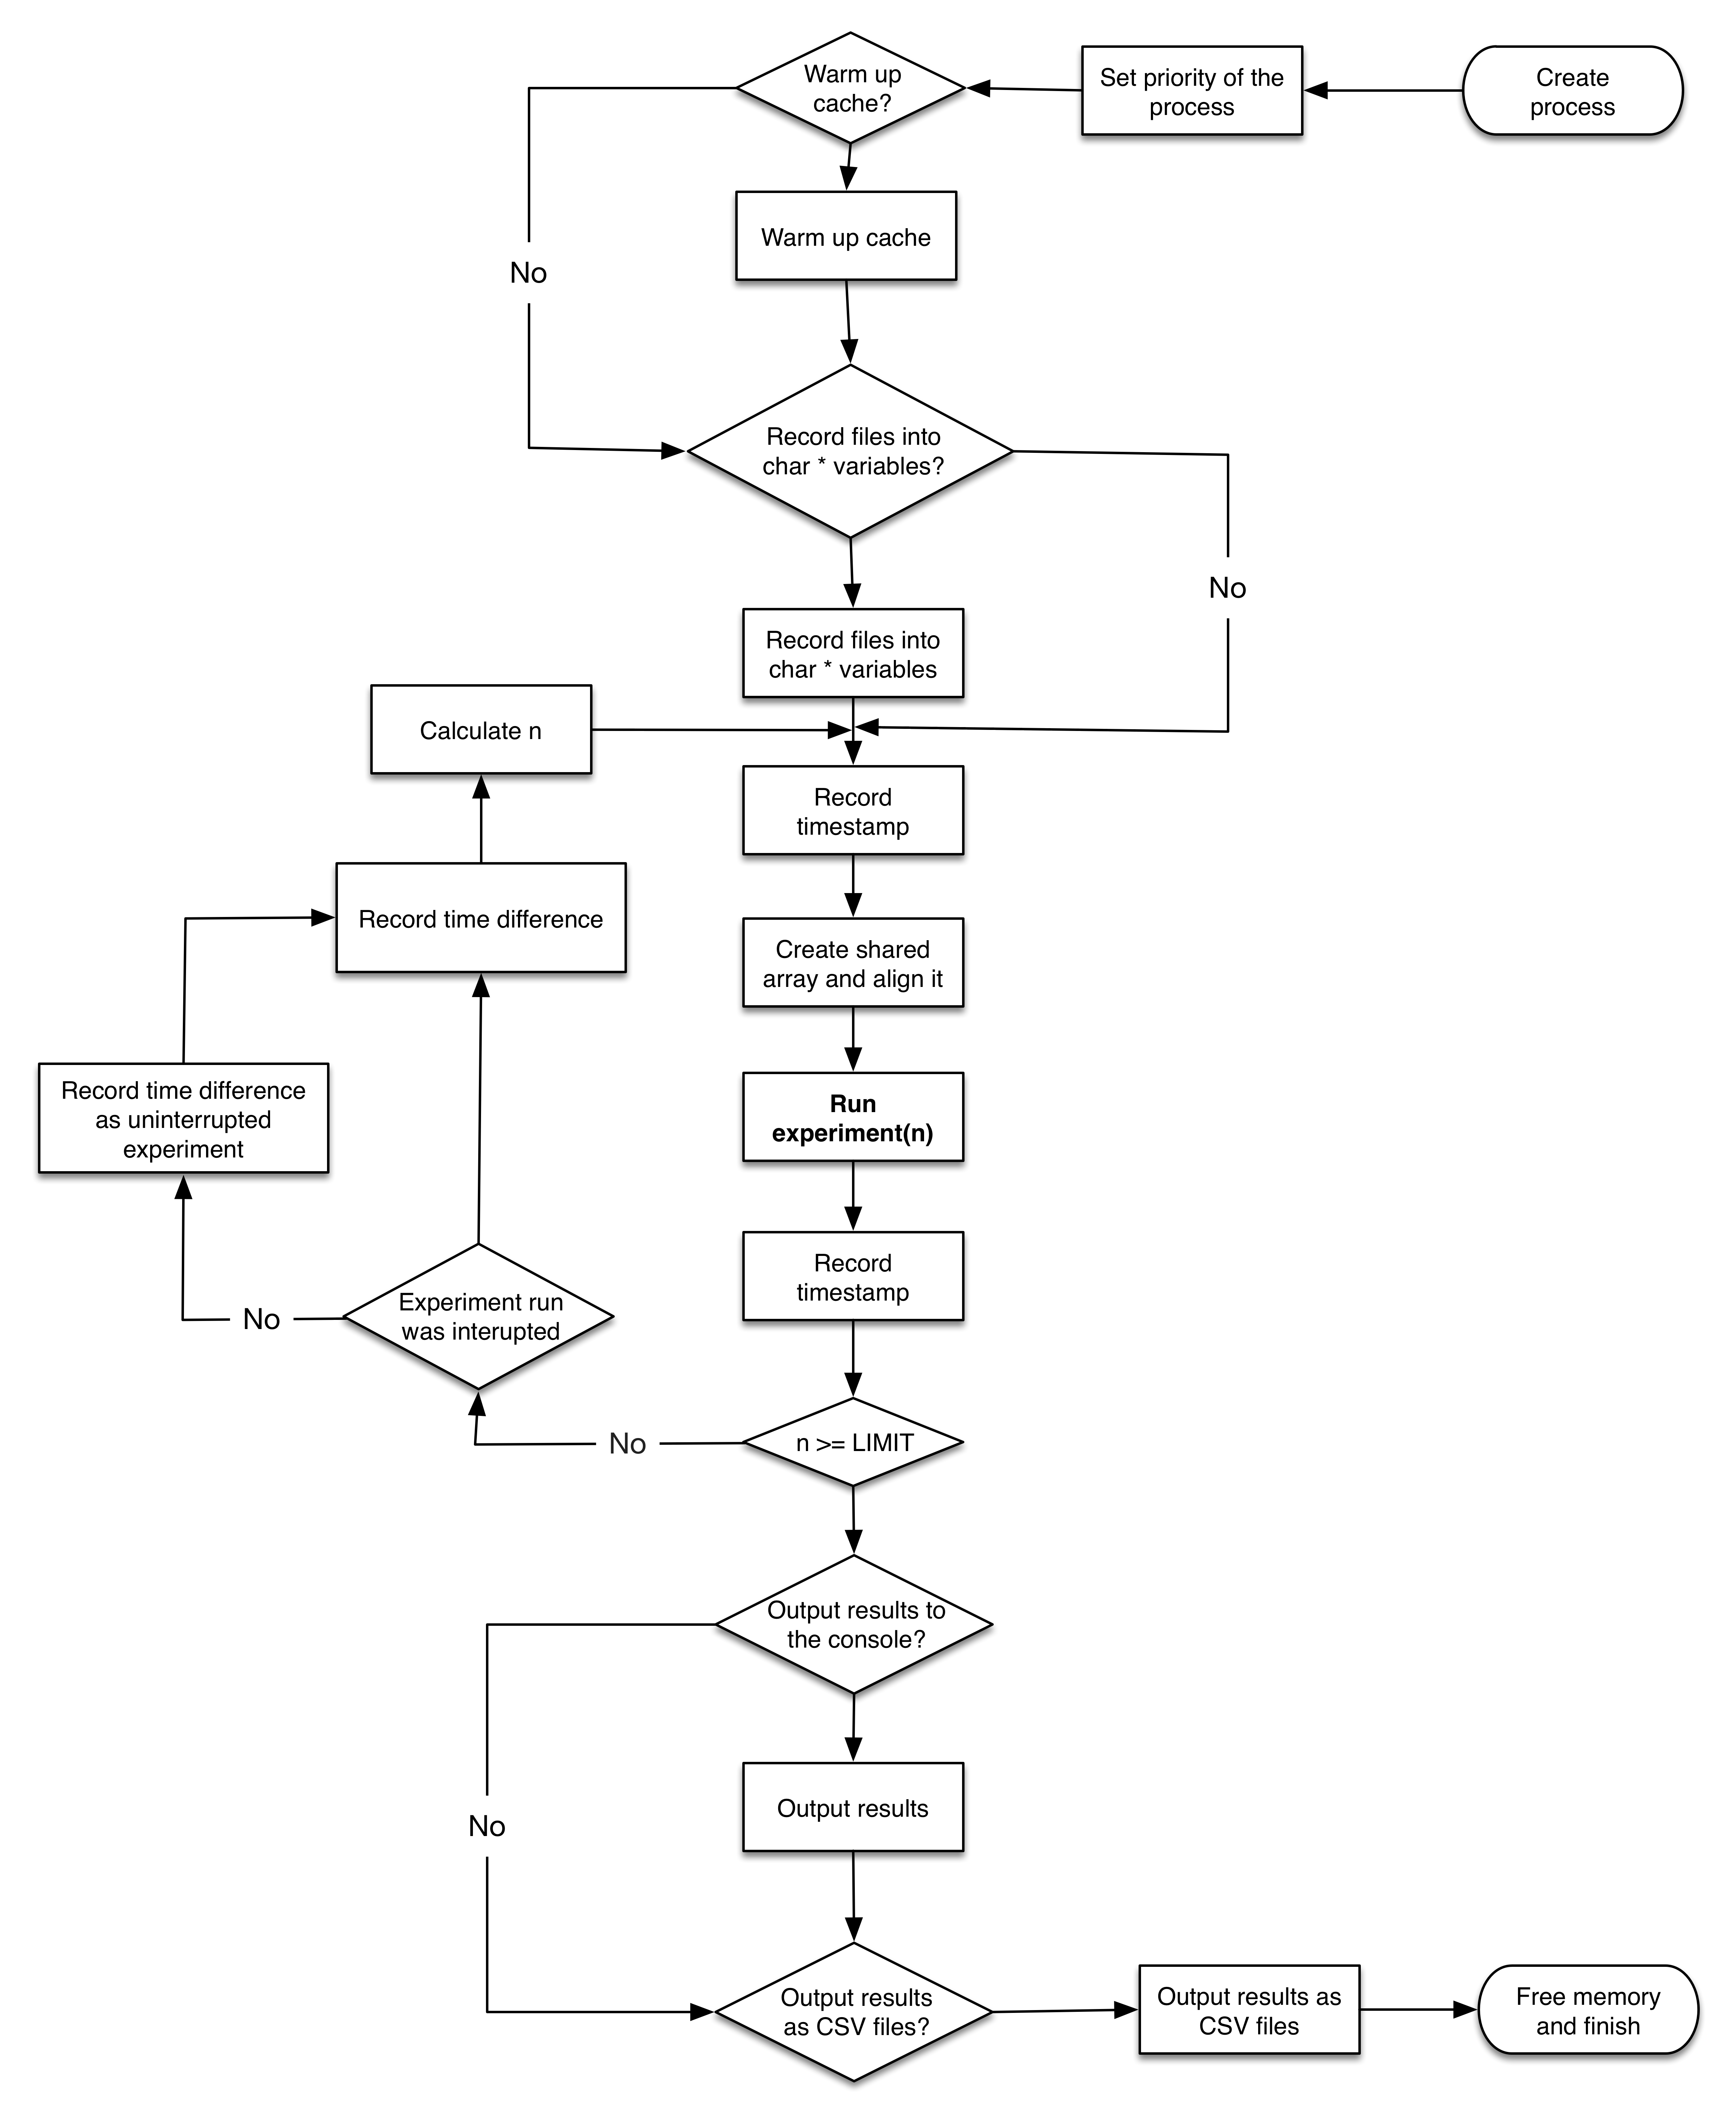
\includegraphics[width=145mm]{4/flow_experiment.png}
\caption{A diagram showing the flow of the process of running an experiment}
\label{flowExperiment}
\end{figure}

The rest of the chapter describes the proposed solution in details.

\section{Organisation of Solution}
\label{fileStrcture}

Even though the structure of the solution is a low-level detail, it is presented in the beginning of the chapter since specific files are referenced throughout the chapter. The C language was used because it has support of working with hardware and kernels of Operating Systems (e.g. by means of the Assembly language), as well as the fact that C does not impose high-level programming structures, such as tools that facilitate the object oriented programming paradigm (like in C++). Additionally, the hardware that was chosen for running experiments is capable of compiling and running programmes written in C without any additional configuration.

All files with the solution described in this section may be found in a folder \textit{``src"}\footnote{\url{https://github.com/Hollgam/cache-mt/tree/master/src/}}. Additional testing programmes are located in other folders, which are referenced when the programmes are discussed. The main files are listed below:

\begin{description}
  \item[clock\_gettime\_mac.c] The implementation of \textit{clock\_gettime(3)} for Mac OS.\footnote{\url{https://github.com/Hollgam/cache-mt/tree/master/src/clock\_gettime\_mac.c}}
  \item[clock\_gettime\_mac.h] The header file for the implementation of \textit{clock\_gettime(3)} for Mac OS.\footnote{\url{https://github.com/Hollgam/cache-mt/tree/master/src/clock\_gettime\_mac.h}}
  \item[conf.h] The configuration file. A number of constants that alter behaviour of the experimental environment are defined in the file.\footnote{\url{https://github.com/Hollgam/cache-mt/tree/master/src/conf.h}}
  \item[experiments.c] The implementation of the experiments.\footnote{\url{https://github.com/Hollgam/cache-mt/tree/master/src/experiments.c}}
  \item[experiments.h] The header for the implementation of the experiments.\footnote{\url{https://github.com/Hollgam/cache-mt/tree/master/src/experiments.h}}
  \item[file\_worker.c] The implementation of a number of functions that support file I/O.\footnote{\url{https://github.com/Hollgam/cache-mt/tree/master/src/file\_worker.c}}
  \item[file\_worker.h] The header for the implementation of a number of functions that support file I/O.\footnote{\url{https://github.com/Hollgam/cache-mt/tree/master/src/file\_worker.h}}
  \item[hr\_timer.c] The cross-platform high-resolution timer for performance measurements.\footnote{\url{https://github.com/Hollgam/cache-mt/tree/master/src/hr\_worker.c}}
  \item[hr\_timer.h] The header for the cross-platform high-resolution timer for performance measurements.\footnote{\url{https://github.com/Hollgam/cache-mt/tree/master/src/file\_worker.h}}
  \item[makefile] Makefile\footnote{\textit{Makefile} is a description file used by the make utility that creates executable files based on the source code and libraries.} for the project.\footnote{\url{https://github.com/Hollgam/cache-mt/tree/master/src/makefile}}
  \item[test\_env.c] A number of functions that support the experimental environment.\footnote{\url{https://github.com/Hollgam/cache-mt/tree/master/src/test\_env.c}}
  \item[test\_env.h] The header for the experimental environment.\footnote{\url{https://github.com/Hollgam/cache-mt/tree/master/src/test\_env.h}}
  \item[test.c] The main entry point of the programme. It prepares the experimental environment and executes the experiments.\footnote{\url{https://github.com/Hollgam/cache-mt/tree/master/src/test.c}}
  \item[test.h] The header for the main entry point.\footnote{\url{https://github.com/Hollgam/cache-mt/tree/master/src/test.h}}
\end{description}

Additional programmes written to test various aspects of the work of CPUs that are mentioned throughout this chapter may be found in other directories: \textit{test\_clockgettime}, \textit{test\_pagefault\_fopen}, \textit{test\_rdtsc}, and \textit{test\_time\_interrupt}.

\section{Experiments}
\label{experimentsDesign}

Two cycle- and three application-level experiments were designed to receive data on latency of different levels of cache, provide a framework to verify the model, and estimate an impact of scheduling on the speed of multi-threaded programmes. Different buffer sizes (amount of exchange data) are used in all experiments; it allows to measure the impact of different levels of memory on inter-thread communication. All experiments are described in the files \textit{experiments.h}\footnote{\url{https://github.com/Hollgam/cache-mt/tree/master/src/experiments.h}} and \textit{experiments.c}\footnote{\url{https://github.com/Hollgam/cache-mt/tree/master/src/experiments.c}}. The following experiments were designed in the project (they are described in the rest of this section):

\begin{description}
  \item[Experiment 0] A base case scenario where memory is stored in CPU registers is discussed. Latency of register-memory is measured.
  \item[Experiment 1] Latency and throughput of all levels of cache is measured.
  \item[Experiment 2] Both the sending and the receiving threads are pinned to a single core (with ID 0).
  \item[Experiment 3] The sending and the receiving threads are pinned to two different cores on the same chip (with IDs 0 and 1).
  \item[Experiment 4] The sending and the receiving threads are pinned to cores on two different chips (with IDs 0 and -1).
\end{description}

\subsection{Cycle-Level Experiments}
\label{design_cycle_level}

Two cycle-level experiments were designed to be executed within the scope of this project. The benchmarking tools described in section \ref{sec:benchmarks} were not used because they do not take timer interrupts and other events that take place in a real-world setting into account. The experiments were created to receive values of latency and throughput of different levels of memory to be applied to the model described earlier.

\subsubsection{Experiment 0}

Experiment 0 is used to measure latency of CPU registers. In Experiment 0 a variable \textit{register long x} is declared to be placed into one of the registers. A different variable \textit{long y} is created, but not as a register-variable. Then, a value of \textit{y} is assigned to \textit{x}. The amount of time that these three operations take is measured. It is considered to be latency of CPU registers. Refer to listing \ref{listingExperiment0} for a source code of the experiment.

\begin{lstlisting}[
language=C,
caption={Experiment 0: measuring latency of registers},
label={listingExperiment0}
]
/*
 * EXPERIMENT 0
 *
 * Measuring latency of registers.
 */
void experiment_0() {
	register long x = 10;
	long y = 0;
	x = y;
}
\end{lstlisting}

\subsubsection{Experiment 1}

Experiment 1 is utilised to measure latency of cache and main memory. It is a simple write-read programme that writes data into a cache and reads it back. A source code of Experiment 1 may be found in listing \ref{listingExperiment1}. An array \textit{long *testAr} is created and aligned. It is used to store data that is written and read. Then, in a for-loop  \textit{n}, all elements are written to the array, and right after that they are read back. Measuring the amount of time that these operations take allows to find the write-read cost of a cache. All allocated memory is then freed and the function is terminated.

\begin{lstlisting}[
language=C,
caption={Experiment 1: measuring latency of cache},
label={listingExperiment1}
]
/*
 * EXPERIMENT 1
 *
 * Measuring cycle-level latency.
 */
void experiment_1(int n) {
	// Aligned array for manipulating data
	long *testAr = align_long_array(sizeof(long) * n); 
	long testLong = 0; // 4 bytes of data
	int i;
	
	// Write and read 1 byte n times
	for (i = 0; i < n; i++) {
		testAr[(int) n] = LONG_TO_ADD; // Write 1 byte
		testLong += testAr[(int) n]; // Read 1 byte
	}
	free(testAr);
}
\end{lstlisting}

These experiments require very high level of precision since they deal with cases that can last for only a few nano-seconds. Special care was taken to prepare the experimental environment, which is described in the sections of this chapter above.

\subsection{Application-Level Experiments}
\label{app_design}

Similarly to the ``Client -- Server" experiment conducted in \cite[p.~63]{Bazilinskyy2013}, all application-level experiments were modelled as client -- server integer addition programmes. By performing such simple arithmetic operation, data can be communicated between threads, yet its implementation is not difficult. Three applications for three different patterns of inter-thread communication in the multi-core environment (as described in section \ref{taxonomy}) were developed.

\subsubsection{Experiments 2 -- 4}

Source code of all of these three experiments is practically identical. These experiments measure latency in three types of inter-thread communication, as described in section \ref{taxonomy}. A listing of one of the application-level experiments where two threads are assigned to the same core (Experiment 2) may be found in appendix \ref{app:listingExperiment2}. All experiments are described by three functions: an entry function and two functions that are executed by POSIX-threads. Refer to figure \ref{flow_threads_app_experiment} for a visual description of the interaction between threads in an application-level experiment, Experiment 3 is taken as an example. An array \textit{testAr} of type \textit{long} and of size \textit{n} is created as the first stage in the entry function \textit{void experiment\_2(int n)}; the entry functions for Experiment 3 and Experiment 4 are called \textit{void experiment\_3(int n)} and \textit{void experiment\_4(int n)} respectively. As was discussed in section \ref{OSinterference}, the arrays that are shared between threads are allocated with cache line alignment. A mutex is then initialised. This synchronization primitive is used to synchronise access to the shared array. A function \textit{pthread\_yield(3)} is utilised to force the writing thread to relinquish the CPU.

\begin{figure}[ht!]
\centering
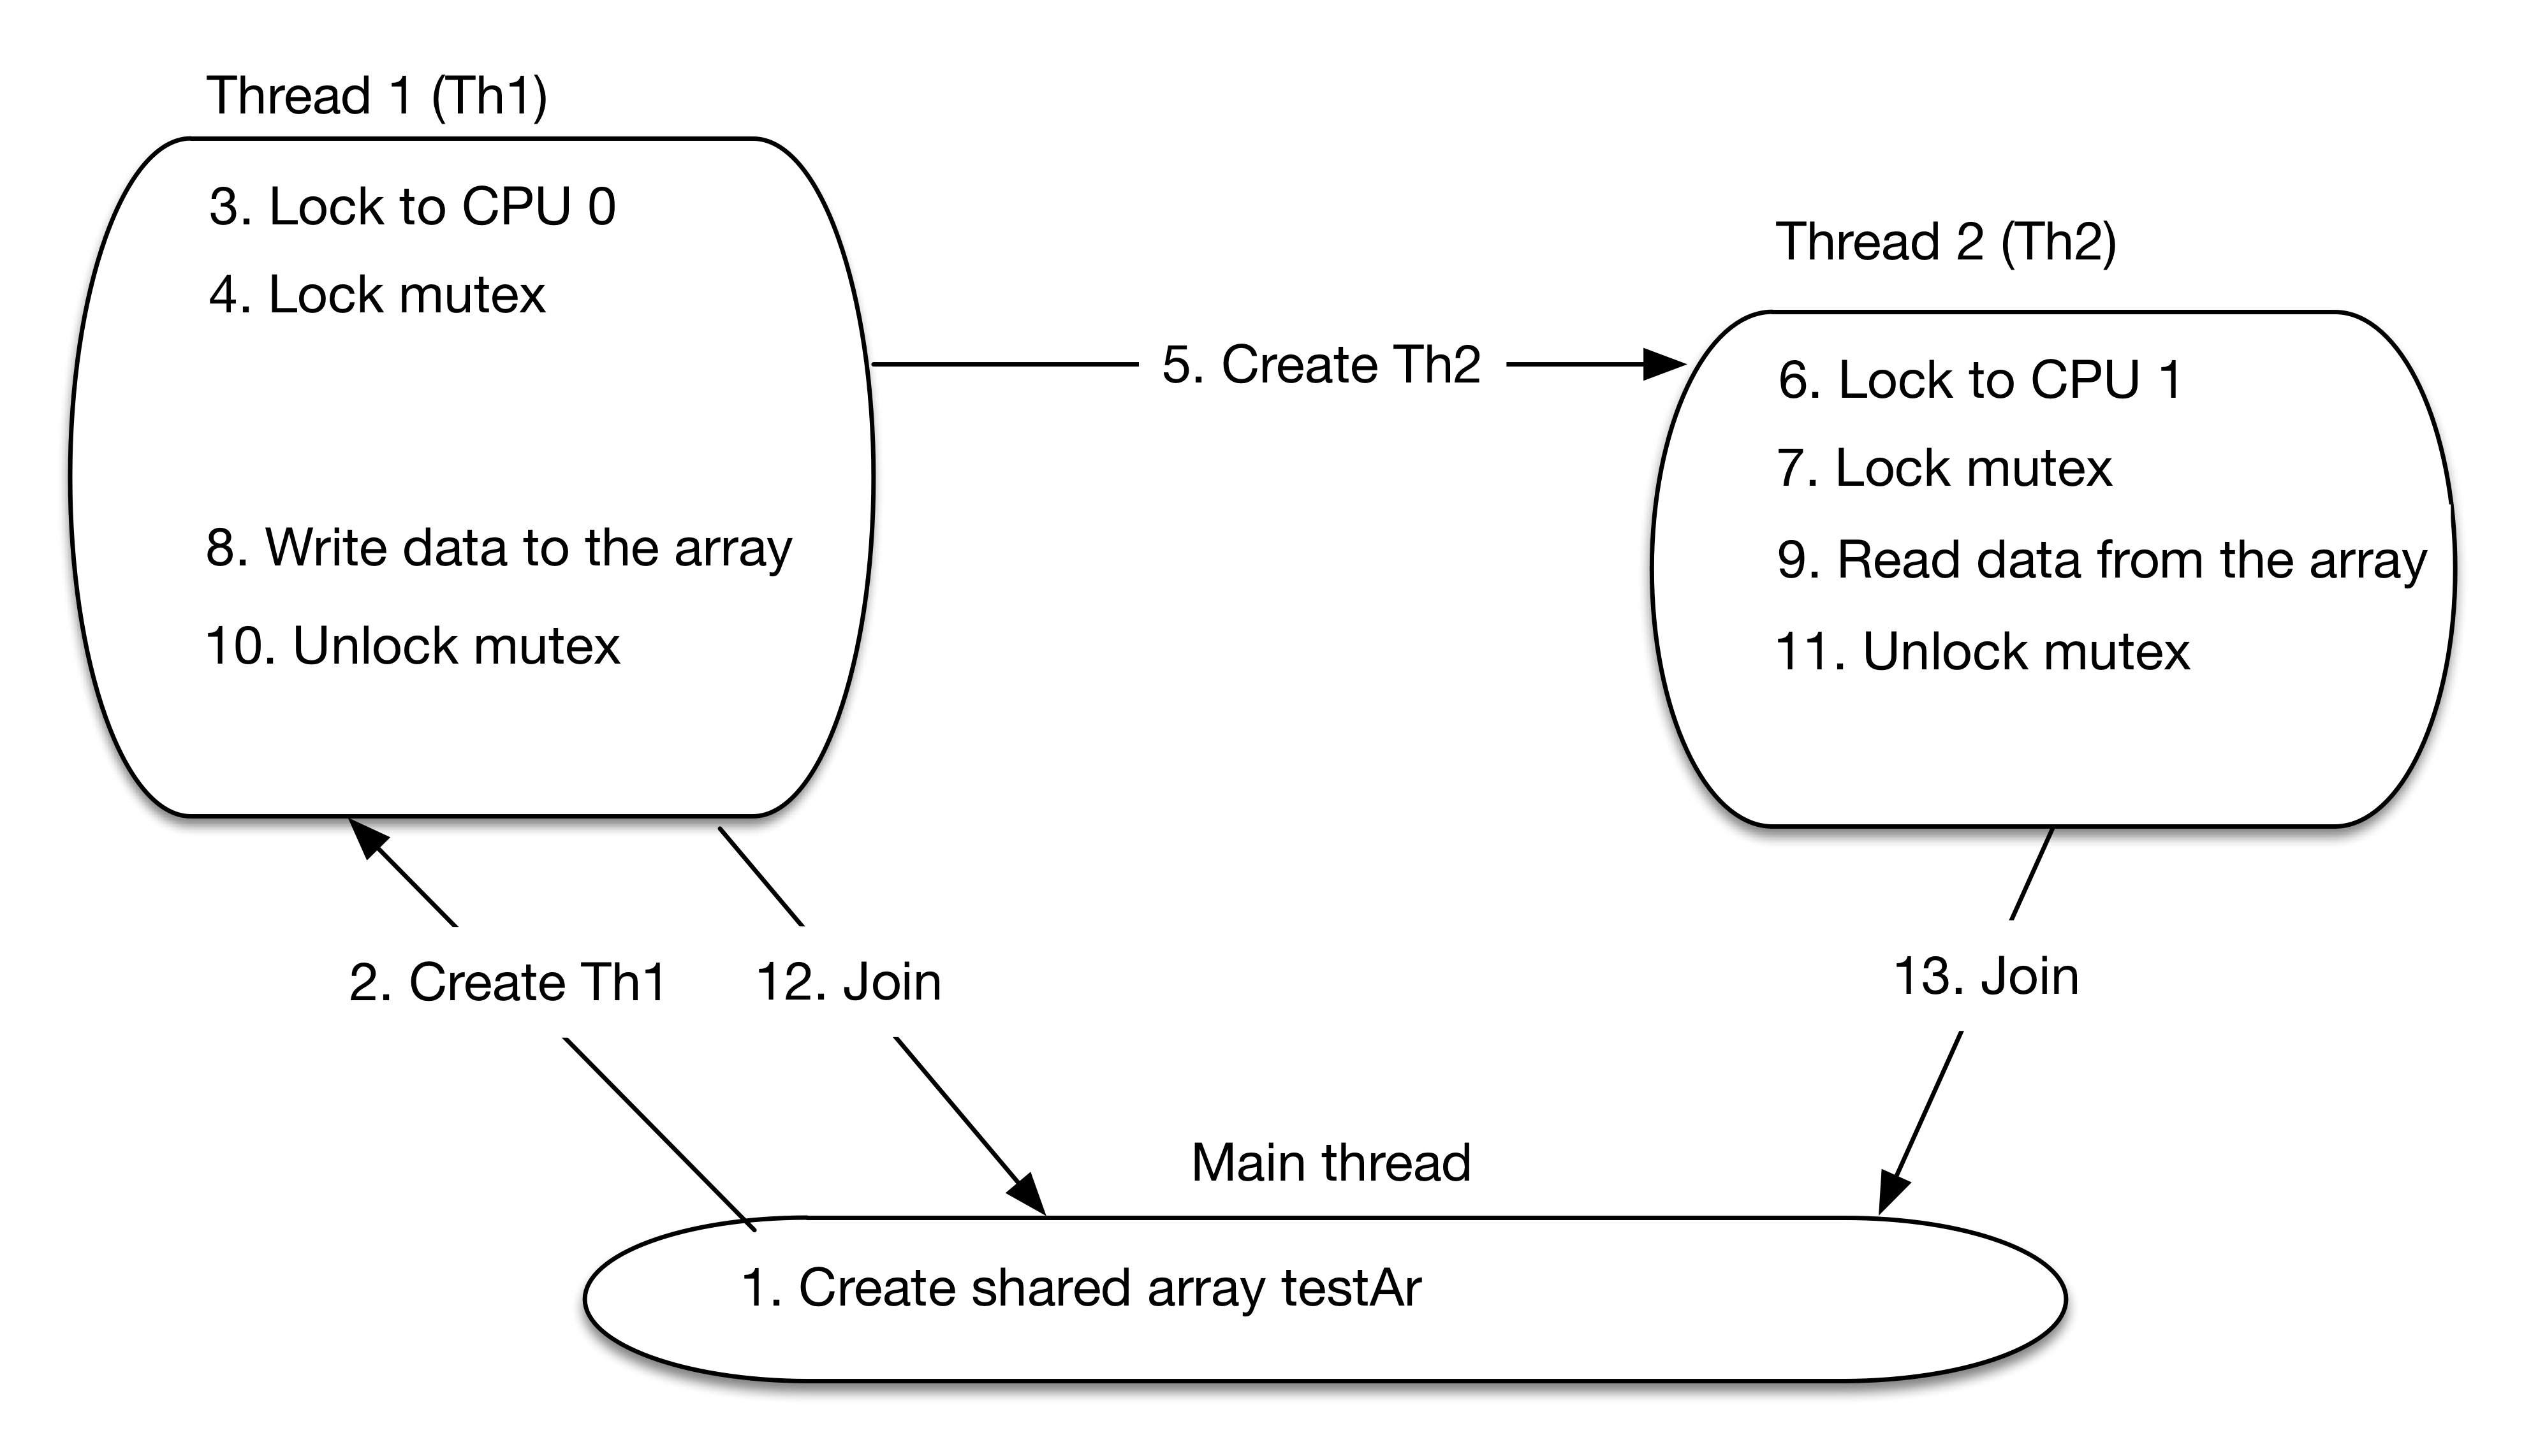
\includegraphics[width=145mm]{4/flow_threads_app_experiment.png}
\caption{A diagram showing the interactions between threads in Experiment 3}
\label{flow_threads_app_experiment}
\end{figure}

The first thread that plays a role of a writer is opened in the entry function, but, before it can be created certain, information needs to be wrapped in a structure so that it can be passed to a function that is to be executed from the new thread. Such ``walk-around" must be used because the \textit{pthread\_create()}\footnote{\url{http://man7.org/linux/man-pages/man3/pthread_create.3.html}} function that has to be called to create a new POSIX-thread can only take a single argument that can be passed to a function that is executed in the thread. Refer to a listing \ref{argStruct} for the definition of the structure. It stores the following information: 1) the ID of an experiment; 2) the size of data that is handled in the current iteration of the experiment; 3) a pointer to the array that is shared between threads.

\begin{lstlisting}[
language=C,
caption={A structure used to pass multiple arguments to the \textit{pthread\_create()} function},
label={argStruct}
]
/*
 * Structure used for a wrapper function used in pthread_create.
 */
struct argStructType {
	int experimentId; // ID of an experiment.
	int n; // Size of data handled in the experiment.
	long * testAr; // Pointer to a shared between
	               // threads structure.
};
\end{lstlisting}

The structure is passed to the thread where it is unwrapped at the entry to the function that is run in the thread \textit{void *e2\_pthread\_main1(void * argStruct)}; functions that are run from the writing threads in the Experiment 3 and the Experiment 4 are called \textit{void *e3\_pthread\_main1(void * argStruct)} and \textit{void *e4\_pthread\_main1(void * argStruct)} respectively. The mutex is then locked.

The second thread is created from the function that is run in the first thread \textit{void *e2\_pthread\_main2(void * argStruct)}; functions that are run from the reading threads in the Experiment 3 and the Experiment 4 are called \textit{void *e3\_pthread\_main2(void * argStruct)} and \textit{void *e4\_pthread\_main2(void * argStruct)} respectively. After that data is written into the shared array (by the first thread), and the mutex is unlocked in the first thread.

Similarly, the wrapped structure is passed to the second thread when it is created. The structure is unwrapped at the entry to the thread function, the mutex is then locked. Now when the mutex is locked and the first thread is prevented from accessing the shared data, contents of the shared array are read by the ``reader" (second) thread. The mutex is then unlocked in the second thread. Finally, both threads are joined by calling the \textit{pthread\_join()} function for each thread. Then, memory is freed and the mutex is destroyed.

\subsection{Organisation of Experiments}
The experiments are run with arrays up to $2^{24} * 8 = 134217728$ bytes (128 MB) in size. Such upper bound was chosen because it is larger than the Level 3 cache size in the Xeon E5-2695 v2, which is the size of the largest cache available across the systems used for executing the experiments. This figure is important because once the buffer contains more data that can fit into the largest cache, data is written into main memory, and caches no longer have impact on the speed of execution. Running experiments that share more data that can fit in the caches allows to measure latency of accessing main memory as well.

\begin{lstlisting}[
language=C,
caption={Function for choosing the length of an experiment},
label={listingCalculateN}
]
long calculate_n(long n) {
#ifdef MORE_EXPERIMENTS
    // Run a lot of experiments
	if (n < 100) {
		n *= 2.0;
	} else if (n > 100 && n < 1000) {
		n += 20;
	} else if (n > 1000 && n < 10000) {
		n += 200;
	} else if (n > 10000 && n < 100000) {
		n += 2000;
	} else if (n > 100000 && n < 1000000) {
		n += 20000;
	} else if (n > 1000000 && n < 10000000) {
		n += 200000;
	} else if (n > 10000000 && n < 100000000) {
		n += 2000000;
	} else {
		n *= 2.0;
	}
	return n;
#else
    // Or just multiple a number of bytes
    // in the iteration by two.
	return n * 2.0; 
#endif
}
\end{lstlisting}

The value of the only parameter -- the size of the array shared among threads -- is calculated in a function \textit{calculate\_n(long n)} that may be found in the file \textit{test\_env.c}\footnote{\url{https://github.com/Hollgam/cache-mt/tree/master/src/test\_env.c}}. This function ensures that samples of latency are taken uniformly. Refer to listing \ref{listingCalculateN} for a source code of that function. If a constant \textit{MORE\_EXPERIMENTS} is not defined, measurements are taken for the array of the size that is calculated as being a power of 2 (\textit{return n * 2.0}).

\begin{lstlisting}[
language=C,
caption={A function for assigning a thread to a particular processor core},
label={listingPinToCore}
]
// Pin thread to a particular core
int pin_thread_to_core(int coreId) {
	int num_cores = sysconf(_SC_NPROCESSORS_ONLN);
	if (coreId < 0 || coreId >= num_cores)
		return EINVAL;

	cpu_set_t cpuset;
	CPU_ZERO(&cpuset);
	CPU_SET(coreId, &cpuset);

	pthread_t current_thread = pthread_self();
	return pthread_setaffinity_np(current_thread,
	    sizeof(cpu_set_t), &cpuset);
}
\end{lstlisting}

A function \textit{int pin\_thread\_to\_core(int coreId)}\footnote{\url{https://github.com/Hollgam/cache-mt/tree/master/src/experiments.c}} for assigning threads to particular processor cores was also designed and developed. Refer to listing \ref{listingPinToCore} for a source code of the function. It utilises standard POSIX functionality that allows to receive a number of cores available in the system, such information is stored in a variable \textit{num\_cores}. A function \textit{pthread\_setaffinity\_np()} is then used to assign a current thread to a core with a given by a parameter \textit{coreId} core.

\section{Configuring Experimental Environment}
\label{design_env}

The rest of this chapter discusses common issues that are related to all experiments discussed in the previous section. A number of problems had to be faced while executing experiments. Solutions to these problems are outlined.

This section describes the experimental environment and outlines main difficulties that the author had to face to successfully run experiments and receive results that meet the requirements on precision and accuracy. The experimental environment can be configured by adjusting values in the file \textit{conf.h} \footnote{\url{https://github.com/Hollgam/cache-mt/tree/master/src/conf.h}}. A number of constants are declared in that file. By adjusting C's preprocessor macros that are defined in various places throughout the solution, one may configure the behaviour of the experimental environment.

All experiments are executed \textit{TIMES\_RUN\_EXPERIMENT} times. Each run of the experiment consists of a number of sub-experiments that are executions of the experiment with specific values given to the variable -- size of data shared between threads, if any -- that declares a number of times that each sub-experiment needs to be run. It is is defined by \textit{TIMES\_RUN\_SUB\_EXPERIMENT}. The values of these parameters were chosen through experimentation. Both of these values may be found in the \textit{conf.h} file.

\subsection{Avoiding Overhead from Operating System}
\label{OSinterference}

Both servers used in the study (refer to section \ref{sec_hardware}) work with Linux distributions. At the time of designing experiments, the server powered by Intel Xeon E5-2695 v2 processors\footnote{The server is referred as \textit{Xeon E5-2695 v2} in this document, unless stated otherwise.} was running SUSE Linux Enterprise Server 11\footnote{\url{https://www.suse.com/products/server/}}; the server based on Intel Xeon 5130\footnote{The server is referred as the \textit{Xeon 5130} in this document, unless stated otherwise.} was operated by Debian GNU/Linux 7\footnote{\url{https://www.debian.org/releases/wheezy/}}. Both of these distributions are identical in the areas that are relevant to this project, both of them are powered by the Linux kernel of version 3 (refer to table \ref{xeonTable}).

Before the design stage an alternative Operating System was also considered: BackTrack Linux\footnote{\url{http://www.backtrack-linux.org/}}. This version of Linux focuses on security and network and its authors claim that it is the ``highest rated and acclaimed Linux security distribution to date". Usage of this version of Linux can potentially present an environment with less overhead. The OS on the Xeon 5130 could be reinstalled; a number of tests with BackTrack Linux were performed by the author on his laptop, but no considerable advantages compared to Debian GNU/Linux 7 were found. The OS that powers Xeon E5-2695 v2 could not be altered, so a possibility of utilising a different Linux distribution for running experiments on that machine could not be considered.

The experimental environment is capable of setting the higher than default priority for the programme thread. It allows to eliminate overhead caused by the experiments being rescheduled by the scheduler. This is achieved with the \textit{setpriority} function\footnote{\url{http://linux.die.net/man/3/setpriority}} that sets the nice value\footnote{A \textit{nice} utility assigns a process with a particular priority, which gives the process either more or less CPU-time, compared to other processes registered in the system.} \cite{citeulike:200722} of the process. All experiments are assigned with higher than default priority. Refer to \ref{listingSetPriority} for the source code with the call of the function with passing appropriate arguments.

\begin{lstlisting}[
language=C,
caption={Setting higher priority of the process},
label={listingSetPriority}
]
int set_highest_process_priority(void) {
	setpriority(PRIO_PROCESS, 0, -20);
	return 1;
}
\end{lstlisting}

% Additionally, a possibility of running experiments as real-time processes \cite{Kernel.org2012} was investigated. However, it was learnt that such behaviour is not supported by the Xeon 5130 and enabling support for user-defined real-time processes would involve recompiling Linux with a modified kernel. It was decided that within the scope of the project such alteration of the OS would not be reasonable. The account that was used to run experiments on the Xeon E5-2695 v2 did not allow for such system-level changes to take place.

Then, a technique of \textit{warming up} cache was utilised in the experimental environment. The ``warm-up" is necessary to avoid receiving false data that is obscured by the interference of cache, as was learnt in the previous project \cite{Bazilinskyy2013}. Without the warm-up, incorrect time measurements would be received in the experiments, since caches would be have to be invalidated before being loaded with appropriate data. A few published papers were investigated, for example \cite{Luo2004}, but it was not possible to find a sufficient number of resources on the ways of performing cache warm-up ``intelligently". The authors of \cite{Luo2004} suggested using heuristics for the warm-up of caches in microprocessors. The heuristics is received by analysing the number of instructions in each sample of code. The proposed method for choosing heuristics is reasonable, but it was concluded that implementation of such technique would not give any noticeable advantage for running the relatively small-scale experiments designed within the scope of the project. The ``warm-up" is achieved by running one iteration of each experiment once before actually conducting the experiments, similarly to what is described in a much older publication \cite{D.Muntz1991}.

\begin{lstlisting}[
language=C,
caption={Alignment of data},
label={listingAlignmentData}
]
// Return a pointer to an aligned array of longs
long * align_long_array(int size) {
#ifdef ALIGN_DATA
    int cacheLine = 64 * 2;
	long x = malloc(size + cacheLine);
	if (x == NULL) { // Array for manipulating data
		printf("Error with allocating space.\n");
		exit(1);
	}
	return (unsigned long *) ((unsigned long long)
	    (x + cacheLine) & 0xFFFFFFE0);
#else
	return malloc(size);
#endif
}
\end{lstlisting}

Then, all data that is shared among threads and is used in the inter-thread communication is aligned on the initialisation stage. Alignment is done to prevent cache misses, which affect performance. Panda P.R. in his papers \cite{Panda1999} and \cite{RanjanPanda1997} together with other researchers discuss the method of alignment, which involves the insertion of ``dummy" data into allocated for a certain variable space. In this project a more simplified approach was taken, where a function receives a pointer to an array of type \textit{long} and simply aligns it by a number of bytes that correlate to the size of one cache line. Refer to listing \ref{listingAlignmentData} for a snippet of C code that performs alignment of data on both the Xeon 5130 and the Xeon E5-2695 v2s. A preprocessor directive \textit{\#ifdef ALIGN\_DATA} checks if a global variable \textit{ALIGN\_DATA is defined}, which indicates that alignment of data must be performed.

Finally, \textit{-O0} flag is used when experiments are compiled with the \textit{gcc} compiler. It ensures that the lowest level of compiler optimisation is used.

\subsection{Measuring Interrupts and Minor and Major Page Faults}

There are a number of sources of inaccuracy of time measurements. To eliminate the overhead imposed by them, the occurrence of the following events is monitored by the experimental environment: minor and major page faults and interrupts. The occurrence of context switches is not traced because, as was learnt, they always occur when interrupts take place. None of these events are desired as all of them take relatively long time to execute and can potentially make low-level experiments invalid.

A page fault can occur when a CPU attempts to access a page that resides in the virtual address space, but cannot be found in physical memory. Such events are normally handled by the memory management unit (MMU) making the required page accessible in physical memory. Attempts to access pages that do not exist are tolerated as ``illegal access errors" and may result in the termination of a programme. There are two types of page faults: minor and major. Minor page faults occur when the page is loaded into physical memory, but the MMU has not marked it as being in the physical memory space. Major page faults happen when the CPU tries to access an address in virtual memory that does not have a page in physical memory assigned to it. The reference to a missing page causes the OS kernel to allocate a page and return back to the MMU. Major page faults have extremely negative impact on the performance of the system, they are much more expensive than minor page faults and they increase latency of memory access dramatically. \cite{rao2008computer}

Another process that regularly takes place in modern-day computers is an interrupt. It is a signal that is emitted when a certain event needs immediate attention and CPU-time. Such high-priority events demand currently executed tasks to be interrupted and scheduled for later execution. When such activity happens, a CPU saves its state and executes an interrupt handler \cite{Mogul1997}. After the interrupt handler finishes its execution, the CPU can continue with execution of the thread that had to be stopped. Interrupts take noticeable amount of time to be finished and can obscure results of experiments that require high precision. A number of different types of interrupts can occur in the system. Time interrupts can be seen each time the internal clock reaches a certain value.

Lastly, a context switch (also known as a task switch) is the switching of the central processing unit from one thread to another. In other words, a context switch\footnote{\url{http://www.linfo.org/context_switch.html}} is a process of the kernel suspending execution of one process and resuming execution of another process that had previously been put on pause. Context switches as well as all aforementioned processes affect multi-threaded programmes \cite{agarwal1992performance}.

An experiment is thought to be invalid if any page faults or interrupts (and consequently context switches) take place during the run of the experiment. Time measurements in such experiments cannot be accurate. One minor page fault per file that is read before starting an experiment is allowed: such page faults rise because of operations that the OS performs when files are read with the \textit{fopen()}\footnote{\url{http://man7.org/linux/man-pages/man3/fopen.3.html}} function. No sources that document such behaviour were found, hence it was proven experimentally with a program \textit{test\_pagefault\_fopen}\footnote{\url{https://github.com/Hollgam/cache-mt/blob/master/test\_pagefault\_fopen/pagefaults\_fopen.c}}. Refer to appendix \ref{app:listingTestPagefault} for the source code of the programme. The output of the programme run on the Xeon 5130 may be seen in a listing \ref{listingOutputPageFaultOpen}.

\begin{lstlisting}[
language=bash,
caption={Results from the experiment that proves that one minor page fault is generated per file-read},
label={listingOutputPageFaultOpen}
]
1st time /proc/interrupts: Before: 209 After: 220
2nd time /proc/interrupts: Before: 222 After: 223
1st time /proc/iomem: Before: 224 After: 225
2nd time /proc/iomem: Before: 226 After: 227
/proc/interrupts changed: Before: 241 After: 244
\end{lstlisting}

The programme \textit{test\_pagefault\_fopen} reads files \textit{``/proc/interrupts"} and \textit{``/proc/iomem"}, which are generated by the Linux kernel and are heavily used in this project. A number of page faults generated across the system is read once before a file is read (written as a number after ``Before:" in the output) and straight after the file is closed (written as a number after ``After:" in the output). A thesis that page faults are generated only after files are read for the first time was suggested. To check this assumption, both files used in the experiments are read twice (results measured when the file is read for the 1$^{\textnormal{st}}$ time are marked with ``1st time", when the file file is opened for the 2$^{\textnormal{nd}}$ time in the same session -- ``2nd time"). The experiment showed that it is not a case. Additionally, a different scenario was tested: when files are changed by the OS between taking measurements of generated page faults. The results from testing this scenario are presented in the last line of the output: three page faults are generated for the file \textit{``/proc/interrupts"}; however, this figure is not constant for different files. A decision was made to disregard results from running experiments where more page faults are generated than a number of files read for measuring data before the start of the experiment.

A number of interrupts that occur during the execution of an experiment is derived by subtracting a sum of all interrupts registered in the system before running the experiment from a sum of all interrupts that can be measured after the experiment has finished. A number of interrupts can be obtained by reading a system file \textit{``/proc/interrupts"} that is generated dynamically on request by the kernel of the OS.

A similar logic is applied to obtaining numbers of page faults (both minor and major) that occur during the execution of experiments: first, one measures a number of page faults that occurred while running an experiment before the execution of the test, then after the experiment has finished. Then, a number of page faults generated before running the experiment is subtracted from a figure that is read after the experiment is no longer running. Such information is generated for each process that is run by Linux individually and may be found in a file \textit{``/proc/PID/stat"}, where \textit{PID} indicates the ID of a process.

The files \textit{``/proc/interrupts"} and \textit{``/proc/PID/stat"} need to be opened for reading information about the numbers of interrupts and page faults recorded prior to running an experiment. The content of these two files is stored in variables of type \textit{char *} and it is read after finishing the experiment. It is done in this way to avoid overhead caused by the analysis of the content of the files for fetching figures of detected interrupts and page faults. Furthermore, before all experiments are run, the content of the files is stored into two ``extra" \textit{char *} variables each time before reading data from them. Such operation is maintained to avoid possible compiler optimisation that may generate additional page faults and prevent receiving accurate results.

\begin{lstlisting}[
language=C,
caption={Measuring time after timer tick or after recording a timer interrupt},
label={listingStartMeasuringTime}
]
#if START_AFTER == TIMER_TICK
	// Start after the timer ticks.
	struct timespec temp_time1, start;

	get_time_ns(&temp_time1);
	get_time_ns(&start);

	while (start.tv_sec == temp_time1.tv_sec &&
	    temp_time1.tv_nsec == start.tv_nsec) {
		get_time_ns(&start);
	}
#elif START_AFTER == TIME_INTERRUPT
	// Start after the time interrupt
	unsigned long long interrupts1 = search_in_file(
	    "/proc/interrupts", "LOC:", 1);
	unsigned long long interrupts2 = search_in_file(
	    "/proc/interrupts", "LOC:", 1);

	while (interrupts1 == interrupts2) {
		interrupts2 = search_in_file(
		    "/proc/interrupts", "LOC:", 1);
	}
	// Calculate the start time
	struct timespec start;
	get_time_ns(&start);
#endif
\end{lstlisting}

To further eliminate a possibility of the Operating System altering the timing results, a number of other precautions were taken. All experiments may be started after a timer tick or after a timer interrupt is recorded in the system. The listing \ref{listingStartMeasuringTime} shows a piece of code in the experimental environment that is responsible for taking a timestamp before running an experiment.

\section{Timing}

\subsection{Measuring Time at Nano-Second Accuracy}
\label{measuringTime}

One of the most challenging aspects of designing the experimental environment for running the experiments that are described in this document was finding a way to measure execution times with enough precision, at a nano-second level. Time can be measured in either nano-seconds or clock cycles\footnote{\textit{Clock cycle} is the amount of time between two adjacent pulses of a processor oscillator.}. A number of options were found and evaluated. This section describes two approaches that were considered.

\subsubsection{Using clock\_gettime(3)}

The first tool that was evaluated for measuring time was the \textit{clock\_gettime(3)}\footnote{\url{http://linux.die.net/man/3/clock_gettime}} function that is provided in most Linux kernels. It is a monotonic function. It is said to be capable of providing measurements of time with nano-second accuracy. The figures of recorded seconds and nano-seconds are stored separately in two 32-bit counters, hence a ``wrap-around" may happen only after many years of the execution time.

The documentation says that \textit{CLOCK\_MONOTONIC} provides ``Clock that cannot be set and represents monotonic time since some unspecified starting point". In other words, it represents the absolute amount of time elapsed since a certain fixed point in the past. It is not affected by the system's clock. \textit{CLOCK\_REALTIME} was also experimented with, but it proved to be less reliable. The reading generated by this clock can be affected by discontinuous jumps in the system time (e.g. the clock is adjusted manually).

The documentation\footnote{\url{http://linux.die.net/man/3/clock_gettime}} associated with this function states that it provides highly-accurate results with nano-second precision. A function \textit{get\_res(3)} was used to find the precision of \textit{clock\_gettime(3)} and, indeed, in cases of both machines utilised in the study \textit{clock\_gettime(3)} does support nano-second precision.

No tools are offered to test the accuracy of this function. A custom programme to check the accuracy of \textit{clock\_gettime(3)} was developed. The application \textit{test\_clockgettime}\footnote{\url{https://github.com/Hollgam/cache-mt/blob/master/test\_clockgettime/clock-gettime\_test.c}} was written to learn whether the amount of overhead of running this function is constant, i.e. if it is capable of outputting the same amount of nano-seconds when the same experiment is run multiple times in the same environment setting. Refer to appendix \ref{app:listingTestClockGetTime} for the source code of the programme. This programme calls \textit{clock\_gettime(3)} 1024 times and records what is returned by the function in each case in an array. Then, it outputs differences between the i$^{\textnormal{th}}$ and the (i-1)$^{\textnormal{th}}$ calls. Refer to \ref{lst:clock_gettime} for an excerpt of the output generated by this programme.

\begin{lstlisting}[
language=bash,
caption={An excerpt from running the \textit{test\_clockgettime} programme on the Xeon 5130},
label={lst:clock_gettime}
]
clock_gettime() ==
90 85 81 81 81 81 82 84 81 81 81 82 81 84 81 81 82 81 81 84 81
82 81 81 81 84 82 81 81 81 81 85 81 81 81 81 82 84 81 81 81 82
81 84 81 81 82 81 81 84 81 82 81 81 81 84 82 81 81 81 81 85 81
81 81 81 82 84 81 81 81 82 81 84 81 81 82 81 81 84 81 82 81 81
81 85 81 81 81 81 82 84 81 81 81 82 81 84 81 81 82 81 81 84 81
82 81 81 81 84 82 81 81 81 81 85 81 81 81 81 82 84 81 81 81 82
81 84 81 81 82 81 81 84 81 82 81 81 81 84 82 81 81 81 81 (...)
\end{lstlisting}

As may be noticed, unfortunately, \textit{clock\_gettime(3)} did not output the same result each time it was called in the testing application. It may be explained by the fact that different underlying instructions may take different amounts of clock-cycles in modern-day CPUs \cite{Granlund2012}. Hence this function cannot be fully trusted for timing experiments that demand high precision. Further, this function uses the \textit{RDTSC} high-frequency timer in its core, so a more direct approach to use that function straight away was considered as an alternative. The overhead of running \textit{clock\_gettime(3)} is also quite large and is equal to 81 -- 90 nano-seconds, which is a big disadvantage of this method.

\subsubsection{Using RDTSC/RDTSCP}

Due to instability of \textit{clock\_gettime(3)} and a relatively large amount of overhead that is associated with calling that function, the \textit{Read time-stamp counter} (RDTSC)\footnote{\url{http://www.mcs.anl.gov/~kazutomo/rdtsc.html}} instruction was chosen as an alternative way to time the experiments. It is an instruction that on x86 and x86-64 platforms can access the Time Stamp Counter (TSC) 64-bit register. As with \textit{clock\_gettime(3)}, the issue of the number reported by \textit{RDTSC} ``wrapping around" is close to being non-existent. The \textit{RDTSC} instruction always returns an increased number until it wraps around. However, in case of, for example, a 2 GHz processor, such behaviour can be seen only after about three centuries.

\begin{lstlisting}[
language=C,
caption={The wrapper function for calling RDTSC with Assembly language},
label={lst:func_rdtsc}
]
/*
 * Use RDTSC to measure time at nanosecond
 * accuracy (if it is not disabled)
 * CPUID == 1 - use CPUID;
 * CPUID == 0 - do not use CPUID.
*/
unsigned long long rdtsc(int CPUID) {
	unsigned long a, b;
	unsigned long long temp;
	if (CPUID)
		__asm__ __volatile__("CPUID\nrdtsc" : "=a" (a),
		    "=d" (b):: "memory", "%ebx", "%ecx");
	else
		__asm__ __volatile__("rdtsc" : "=a" (a),
		    "=d" (b):: "memory", "%ebx", "%ecx");
	temp = b;
	temp = (temp << 32) | a;
	return temp;
}
\end{lstlisting}

\textit{RDTSC} is an Assembly command that loads the current value of the processor's time-stamp counter into the EDX:EAX registers \cite{Faydoc2014}. A wrapper function that calls a piece of inline Assembly code was written. Refer to \ref{lst:func_rdtsc} for a listing with a source code of the function. This function has a single parameter \textit{int CPUID}, which is a flag that indicates whether \textit{CPUID} instruction should be called before invoking the \textit{RDTSC} operation. This instruction is called before \textit{RDTSC} because it prevents out-of-order execution on modern CPUs (a situation when instructions are executed in a different than was programmed order). Invocation of the \textit{CPUID} command serializes the instruction queue. 

The author of \cite{Kankowski2012} states that a combination of \textit{CPUID} and \textit{RDTSC} can provide constant performance, i.e. the overhead associated with invoking these commands is constant. A function \textit{void test\_rdtsc(void)}\footnote{\url{https://github.com/Hollgam/cache-mt/blob/master/test/src/hr\_timer.c}} was built to verify this thesis. Refer to appendix \ref{app:listingTestRDTSC} for a source code of the function. Similarly to the test that was performed to verify the accuracy of \textit{clock\_gettime(3)}, this program calls \textit{RDTSC} 1024 times. Refer to figure \ref{lst:test_rdtsc} for an excerpt from the output of this application when it was run on the Xeon 5130. It outputs what is received from the instruction: large numbers (e.g. 21210592467695670), which represent the amount of ellapsed time. The numbers in square brackets indicate the differences with what was returned from the previous calls of the \textit{RDTSC} instruction (e.g. [336]). Despite what is claimed in \cite{Kankowski2012}, this excerpt clearly shows that RDTSC is not capable of providing constant performance on the Xeon 5130, the test was also executed on the Xeon E5-2695 v2, but the results were largely the same: the overhead was not constant. It may be a case because of the nature of underlying Assembly-commands that take different numbers of clock-cycles to execute on modern CPUs. Any other more reliable sources of information on the nature of \textit{RDTSC} and its performance could not be found.

\begin{lstlisting}[
language=bash,
caption={An excerpt from running the \textit{test\_rdtsc()} function on the Xeon 5130},
label={lst:test_rdtsc}
]
21210592467695670 [336]
21210592467695994 [324]
21210592467696318 [324]
21210592467696642 [324]
21210592467696972 [330]
21210592467697296 [324]
21210592467697626 [330]
21210592467697950 [324]
21210592467698274 [324]
21210592467698604 [330]
21210592467698928 [324]
21210592467699252 [324]
21210592467699594 [324]
21210592467699918 [324]
21210592467700242 [324]
21210592467700566 [324]
21210592467700890 [324]
21210592467701220 [330]
(...)
\end{lstlisting}

The aforementioned test showed that receiving accurate timing information with assistance of RDTSC is a complicated undertaking on its own. In addition to the problem of out-of-order execution of instructions on modern-day CPUs (like those that are used in the study), the clock speed also varies, which leads to the alteration of timing results. In older multi-core systems, the rate returned by \textit{RDTSC} could change differently on different execution units, as they would adjust their clock speeds according to the load.

Another possibility was suggested in one of the white paper from Intel on this topic \cite{Paolini2010}: the \textit{RDTSCP} instruction. The main difference between \textit{RDTSCP} and the standard \textit{RDTSC} instructions is that \textit{RDTSCP} works as a serializing instruction, i.e. the CPU is prevented from reordering instructions around the call to \textit{RDTSCP}. Unfortunately, \textit{RDTSCP} is available only on new processors, and a number of tests showed that it could not be run in the experimental environment designed for this project.

\section{Support for Mac OS}

Because a machine powered by Mac OS X could be easily accessed, this Unix-based OS was also selected as a platform for running the experiments. Most functionality that is supported by Linux is also available in Mac OS. This assumption was not valid in case of the \textit{clock\_gettime(3)} function. A custom-built timer that imitates the behaviour of \textit{clock\_gettime(3)} was designed and developed in the early stage of this project to extend support of Mac OS. Its implementation may be found in the file \textit{clock\_gettime\_mac.c}\footnote{\url{https://github.com/Hollgam/cache-mt/tree/master/src/clock\_gettime\_mac.c}}.

It was speculated that the author's MacBook Air laptop powered by an Intel i7 processor could also be used for running experiments. Then at a much later stage of the project the fact that Mac OS does not support assigning threads to particular cores was discovered. The initial vision of the experimental environment assumed that it would be cross-platform and could be used for running experiments on both Linux-based systems and on Mac OS X. After it was learnt that such vital for the success of the project functionality cannot be achieved by using the standard tools offered on Mac OS, a decision to abandon the cross-platform support was taken. As a result, the proposed system is only partially cross-platform.

\section{Measuring Duration of Interrupts and Minor Page Faults}
\label{design_duration_int_pf}

It is important to know the duration of one time interrupt and a minor page fault, since these events have a big affect on performance of a system that is engaged in inter-thread communication. At first an attempt to retrieve information about the values of duration of page faults, context switches, and interrupts was undertaken. No such data was found for both CPUs used in the experiments.

A programme for testing the duration of an interrupt \textit{test\_time\_int\_pf}\footnote{\url{https://github.com/Hollgam/cache-mt/tree/master/test\_time\_int\_pf}} was written. Refer to appendix \ref{app:listingTestInterrupt} for a listing of the source code of the main function that handles the experiment. Most supplementary functions that handle measuring time and getting information on the numbers of recorded interrupts and page faults are described in this chapter. This application waits until an interrupt is detected and measures a difference between timestamps taken before and after occurrence of the interrupt. Such operation is performed 10 times. Similar actions are taken to record the duration of a minor page fault. Then, the average duration of one interrupt is reported.

\section{Dependability}
\label{dependabilitySection}

This section discusses the aspect of dependability of the proposed solution. This thesis focuses on the impact of cache on data-intensive multi-threaded application. Programmes of this type often have high requirements for security and protection of data: separation of bandwidth in telecommunication systems, accessing data in distributed databases, etc. Speed is an important factor for achieving stable performance of such systems, and the impact of the cache needs to be predictable and quantifiable.

The outlined in the section experiments run directly on the hardware. Execution times are measured by extracting information straight from CPU registers. Therefore, measured data is dependable, provided that the used hardware does not malfunction. Boolean logic is used to test modern-days microprocessors and the probability of using a faulty processor is very small, as the fault tolerance of CPUs is extremely high. Two processors were used to run the experiments, one of which powers a supercomputer in a respected research institute, so the chance of operating a faulty processor becomes even lower.

All experiments were run ten times and the final results are generated from calculating the average values from all runs of the experiments. Moreover, special care was taken to avoid interference from the OS by detecting interrupts and page faults, warming up caches, and starting each experiment after a timer tick / interrupt is recorded.
% ---------------------------------------------------------------------------
%: ----------------------- end of thesis sub-document ------------------------
% ---------------------------------------------------------------------------

